\section{State Properties and Exact Implementation}\label{app:properties}
\begin{proposition}[Invariant state ranges under the implemented updates]
Suppose $k>0$, $\alpha_I,\alpha_C,\alpha_U\geq0$, $q\in[0,1]$, $w\in(0,2)$, and delivered feedback $y\in[0,1]$. Starting from the prescribed bootstrap or insertion state, the hybrid updates preserve $0<I\leq20$, $0\leq C\leq1$, $U\geq0$, and $T\geq0$ at finite event times. Under held inputs and positive corresponding strengths, $I$ and $C$ approach their targets monotonically and $U$ contracts.
\end{proposition}
\begin{proof}
Each update of $I$ or $C$ in Equation~\ref{eq:closed} is a convex combination of its pre-flow value and target because its exponential coefficient lies in $[0,1]$. The importance target lies in $[0.5,2.5)$ and the consistency target in $\{0,1\}$. Insertion has $I=gw\in(0,2)$; duplicate observation caps its positive increment at 20. Consistency observation resets to one and feedback is a convex combination with $y$. Usage flow multiplies a nonnegative value by a nonnegative factor and feedback adds a nonnegative value. Temporal flow adds a nonnegative interval and resets to zero. These operations preserve the asserted ranges by induction over events. The differences from held targets are multiplied by positive decaying exponentials, establishing monotone approach between events. This does not imply monotone task performance or bounded $T$ across an infinite stream.
\end{proof}

\begin{proposition}[Conditional usage bound]
If $\alpha_U k(t)\geq\kappa>0$ while a record is resident, usage increments are at most one, and successive increment times are separated by at least $\delta>0$, then post-increment usage satisfies
\begin{equation}
U_n\leq r^nU_0+\frac{1-r^n}{1-r},\qquad r=e^{-\kappa\delta/20}<1.
\end{equation}
\end{proposition}
\begin{proof}
Between successive increments, the flow contracts usage by at most $r$; hence $U_{n+1}\leq rU_n+1$. Iterating this scalar inequality gives the bound. Additional resets through eviction and reinsertion only lower usage. If strength is zero or increments can accumulate without a positive spacing bound, the uniform bound does not follow. The observed usage of 220 at zero strength is therefore not evidence of numerical instability.
\end{proof}

\paragraph{Rate control and selection discontinuities.}
The state at a fixed time is smooth in a rate on any interval without discrete policy changes. The map from a rate to task outcomes is not smooth in general: when two retention scores cross, a different record can be evicted and all later observations, answers, and feedback-dependent states can diverge. Consequently, neither the smooth vector field nor the finite C1 grid implies a continuous monotone performance frontier. Our operational claim is supported opposing changes at sampled settings.

\paragraph{Why decay rescaling cannot match replacement by itself.}
For fixed observation ages $a_i$, every positive $\lambda$ gives the same ordering of $\exp(-\lambda a_i)$, equivalently $-\lambda a_i$. A fixed-capacity minimum-score eviction policy therefore chooses the same victim under any positive rescaling, except unchanged ties. The implemented replacement control explicitly changes admission, not merely the decay coefficient. The matrix extension also uses a minimum resident age. This distinction is necessary for interpreting the control's name.

\paragraph{Lifetime bookkeeping.}
If each admitted residency is followed to eviction or the evaluation endpoint, summing its observed duration gives $\int_0^T|\mathcal M_t|\,dt$. When the store is always full, this is $KT$. With $E$ evictions and $K$ final right-censored residents, mean observed residency duration is $KT/(E+K)$. Thus matching mean duration and eviction count does not provide two independent controls under full occupancy. Warm-up occupancy, the lifetime distribution, censoring, resident age, and the identities of removed items remain relevant.

\section{Frozen Head and Feature Provenance}\label{app:head}
The head is an affine map from 40 features to three coefficients, not an LNN or recurrent hidden-state model. The first 32 features encode content. The remaining features are: an observation/context event indicator; $\log(1+\Delta)/5$; exponentially decayed query demand for the current key; capped time since its last query; an exponential mean of observed version conflict; mean delivered feedback; most recent delivered feedback; and agreement with the held context. Demand decays with time constant 30. Conflict and feedback running averages are causal. No stable-role flag or reference answer is included.

The earlier development run used four conditions (mixture, feedback noise, misleading feedback, and cyclic demand), with 8 training and 4 validation schedule seeds per condition and capacities 8/12. Noise-related conditions share underlying worlds. The training objective was
\begin{equation}
\mathcal L=(1-A)+0.25(1-\mathrm{SR})+0.25\mathrm{SE}.
\end{equation}
Hard-capacity decisions were trained with REINFORCE, a deterministic fixed-policy baseline, AdamW at 0.003, batches of eight, gradient clipping at one, and sixteen epochs. Validation utility pooled the development conditions and capacities. Initialization was eligible for selection. The selected checkpoints for seeds 11/23/42 are epochs 15/9/14, with validation utilities 0.7467/0.7412/0.7657. These weights precede the validation matrix and were not retrained for any reported B/C batch. This provenance does not make the synthetic content distribution independent of development templates.

In the rule baseline, $(g,w,k)=(2/3,1.5,0.3)$. For learned evolution, $g$ is the insertion gate; it must not be confused with the externally swept $\alpha$. We use a shared strength in C1, single active flow in C2, default strength one in semantic migration, and strengths $\{0,0.25,1,2\}$ in long-horizon stress. All content versions are explicit records. The version ledger persists identifiers after eviction but not content; the query history is also auxiliary metadata outside the slot constraint.

\section{Protocols, Statistics, and Amendments}\label{app:protocol}
\paragraph{Frozen batch design.}
Protocols, checkpoints, random seeds, event streams, full state trajectories, write rejection decisions, censored lifetimes, raw metrics, and statistical comparisons are stored with hashes. The final characterization used 244 mini configurations, each exactly replayed, before 17,568 formal policy trajectories. The current source test suite passes 251 tests. These checks establish implementation and replay consistency, not external validity or absence of every possible modeling bias. Protocols were frozen locally before each formal batch; this was an iterative research project, not an externally registered study blind to all earlier results.

\begin{center}\small
\begin{tabular}{llll}\toprule
Experiment family & Formal worlds & Seeds & Scope\\\midrule
B1-A attribution & 72001--72024 & 11/23/42 & $3$ dynamics $\times3$ pressure cells\\
B2 capacity & 82100--82123 & 11/23/42 & $K=4,8,16,32,64$\\
B3 cycle & 83100--83123 & 11/23/42 & A--B--A with pre-reminder probes\\
B4 corruption & 84100--84123 & 11/23/42 & clean, 10/25/50\%, misleading cue\\
B5 revision & 85100--85123 & 11/23/42 & observed value updates\\
B6 state intervention & 86100--86123 & 11/23/42 & four neutral-state controls\\
B7 integration & 87100--87123 & 11/23/42 & event-only, Euler, query-held cue\\
C1 rate scan & 91100--91123 & 11/23/42 & two settings, two capacities\\
C2 flow attribution & 92100--92123 & 11/23/42 & four flow families, seven strengths\\
C3 semantic replay & 93100--93123 & 11/23/42 & four tasks, two capacities\\
C4 long horizon & 94100--94123 & 11/23/42 & three lengths, two capacities\\\bottomrule
\end{tabular}
\end{center}

The structured matrix uses shared four-record bootstrap states, eight currently active facts, and interleaved observation/query/feedback. Stable facts are periodically queried; two groups of four volatile facts exchange demand. B1-A varies interference pools 2/8/16 and stable/slow/rapid revision schedules. B2 fixes the core identities but scales interference pool size to $2K$, with equal core and interference arrival counts per phase. B3 excludes factual revisions to isolate demand return. B4 shares the same observation and query tapes across corruption rates. C1 mixed and rapid/high use different interference pool sizes and revision settings; an effect across them cannot be attributed to one factor alone.

\paragraph{What is held equal?}
Every policy sees the same exogenous observations, context cues, query times, and corruption draws within a world. Scored feedback is generated only after answering, so identical exogenous streams do not imply identical realized feedback histories. The core synthetic retrieval budget is one answer from the addressed resident key. A new observation creates one capacity decision; a duplicate refresh does not create an extra resident version. Policies may differ in accepted writes and rejections, which are recorded separately from resident replacements. The common implementation includes four state fields even in fixed policies, so multiplying four scalars by capacity is not a measured incremental heap allocation.

\paragraph{Metrics and inference.}
For query set $Q$ and stable subset $Q_s$, $A=|Q|^{-1}\sum_q\mathbf1[\hat a_q=a_q]$, $\mathrm{SR}=|Q_s|^{-1}\sum_{q\in Q_s}\mathbf1[\hat a_q=a_q]$, and $\mathrm{SE}=|Q|^{-1}\sum_q\mathbf1[\hat a_q\text{ is an obsolete value of the queried fact}]$. Missing answers and wrong-fact answers are incorrect but not automatically stale. The lag rule needs at least five queries; an episode with no recovery takes its full horizon. A recovered final query and an unrecovered episode may share the same lag, so recovery success is separately saved. Intervals and tests use paired worlds after averaging the three policy seeds; neither individual queries nor seeds inflate the sample size. C1 corrects 168 endpoint tests, C2 252, C3 80, and C4 90 within their respective batches. These families were not jointly corrected into one universal claim. The archive retains both within-batch and additional across-matrix comparisons where available.

\paragraph{Amendments without policy optimization.}
The semantic replay initially counted unchanged continuation phases as adaptation episodes. Evaluation was corrected to start after observed new-value exposure and to distinguish demand return; the same seeds were rerun, retaining the earlier files. Twelve deterministically selected old/new trajectory replays have identical actions, states, queries, and lifetimes; the changed fields are adaptation episode definitions and derived metrics. The long-horizon prototype repeatedly changed demand but concentrated fact revisions early. Before interpreting formal performance, it was amended to introduce a different observed public value on the first active-fact observation after every subsequent context shift. Prior mini and partial formal files remain in the superseded archive. These are protocol corrections, not evidence of a fully preregistered end-to-end study.

\section{Semantic and Language Transfer Details}\label{app:semantic}
\paragraph{Controlled public-text migration.}
MemOps (revision \texttt{312af65e2c7b}, full hash in the archived protocol) supplies confirmed observation/update quotes. Ten target domains cover browser, keyboard, author, hotel brand, naming preferences, travel, examination date, and storage plan. Four stable controls are sampled from never-revised side facts. Each task has four active targets and sixteen interference identities. Public quotes are reused across 24 schedule worlds; uncertainty thus describes schedule variation, not sampling of independent language corpora. Historical distractors explicitly say they are no longer current, but the adapter has no gold semantic contradiction resolver.

The encoder is frozen \texttt{all-MiniLM-L6-v2}. A new observation hashes its content for duplicate detection. Otherwise its nearest resident embedding is used to reuse a key if cosine similarity is at least 0.65; failing that, a new key is assigned. Reused keys increment the observed arrival version. A query selects the nearest resident embedding's key, then the newest resident version within that key. All thresholds were fixed before formal outcomes. Demand affinity is $\max(0,\cos(x_i,c))$ under the held context cue, replacing the structured binary affinity. The 384-dimensional vector is projected to the same 32 head features. Removed records lose their embeddings; no evicted vector archive can supply answers. The evaluation wrapper's gold identity, value, and stability label are excluded from policy inputs.

Four tasks test preference update, contradictory historical evidence, old-preference revival, and temporary task information. Preference-update and contradiction adaptation include only the observed revised-value queries in the actual update phase; unchanged continuation is not counted as another update. Revival includes a probe before new reminder observations. At capacity sixteen, pre-reminder recall is 17.71\% for \ame versus 98.61\% for frequency, despite \ame's higher aggregate revival accuracy. Mismerge counts track wrong-fact key merging, not false separation of versions. The post-hoc semantic routing audit reports both; its descriptive link rate is conditional on an old value still being resident. It is not a new randomized intervention on the addressing layer.

\paragraph{Conversational transfer protocol.}
The held-out subset comprises 24 LongMemEval questions (four from each of six categories), 24 LoCoMo questions drawn across ten conversations, and 24 NFCats test questions with 200 released training dialogs. Each is evaluated with seven policies and three policy seeds, for 1,512 formal answer records. LoCoMo answers are clustered by conversation; other datasets by question. All NFCats questions share one training history, so uncertainty is conditional on that history. A held-out question is not presented during consolidation.

The memory adapter uses exhaustive spans up to 1,200 characters, capacity 64, top-five retrieval, and a 12,000-character reader budget. The topic signal is a fixed content-projection heuristic, not gold semantic parsing. LongMemEval/LoCoMo provide no correctness feedback during consolidation; NFCats supplies released off-policy dialog feedback. Dated dialogs use days as the time unit, while NFCats uses dialog steps; this time-scale transfer is uncalibrated. These limitations make the transfer study a boundary probe rather than a production memory system comparison.

Answers and blinded evaluation use \texttt{agnes-3.0-flash}, temperature zero, answer maximum 384 tokens, at \url{https://api.agnes-ai.cn/v1}. Rate-limited calls, retries, prompts, raw responses, token usage, and judge-format repairs are saved. LongMemEval/LoCoMo use reference-based binary correctness plus auxiliary token F1. NFCats uses a reference-free 1--5 rubric normalized as $(s-1)/4$; satisfactory response rate uses $s\geq4$. Neither NFCats quality nor its uncertainty should be interpreted as binary QA accuracy. We did not vary the language backend or use a separate judge model. Stale error, stable retention, and adaptation lag are unavailable without suitable labels and are left null, not inferred from generic wrong answers.

\section{Long-Horizon and Computational Diagnostics}\label{app:stress}
The stress generator maintains exact common prefixes at 500, 1,000, and 5,000 events. Following 37 warm-up events, each phase has one context cue and 32 observation/query/feedback triples, hence 97 events. Every complete post-initial phase introduces four active-fact revisions upon their first observation. Each shift has sixteen target queries. The terminal partial episode is excluded from the lag average but retained in raw event metrics. No missing future observation is imputed.

The descriptive collapse indicator is two consecutive 100-event scored windows with accuracy below 10\%. At 5,000 events the fully frozen-state control triggers it in 16/72 trajectories at capacity eight and 2/72 at capacity sixteen; no other tested method does. This indicator does not certify quality: frequency still has substantial stale-answer accumulation. At sixteen slots, its final-window obsolete-resident fraction is 74.31\%, versus 0.039\% for strength one. All state values remain finite. These results concern the finite 28-key test and do not establish infinite-horizon or open-world guarantees.

\begin{figure}[p]\centering
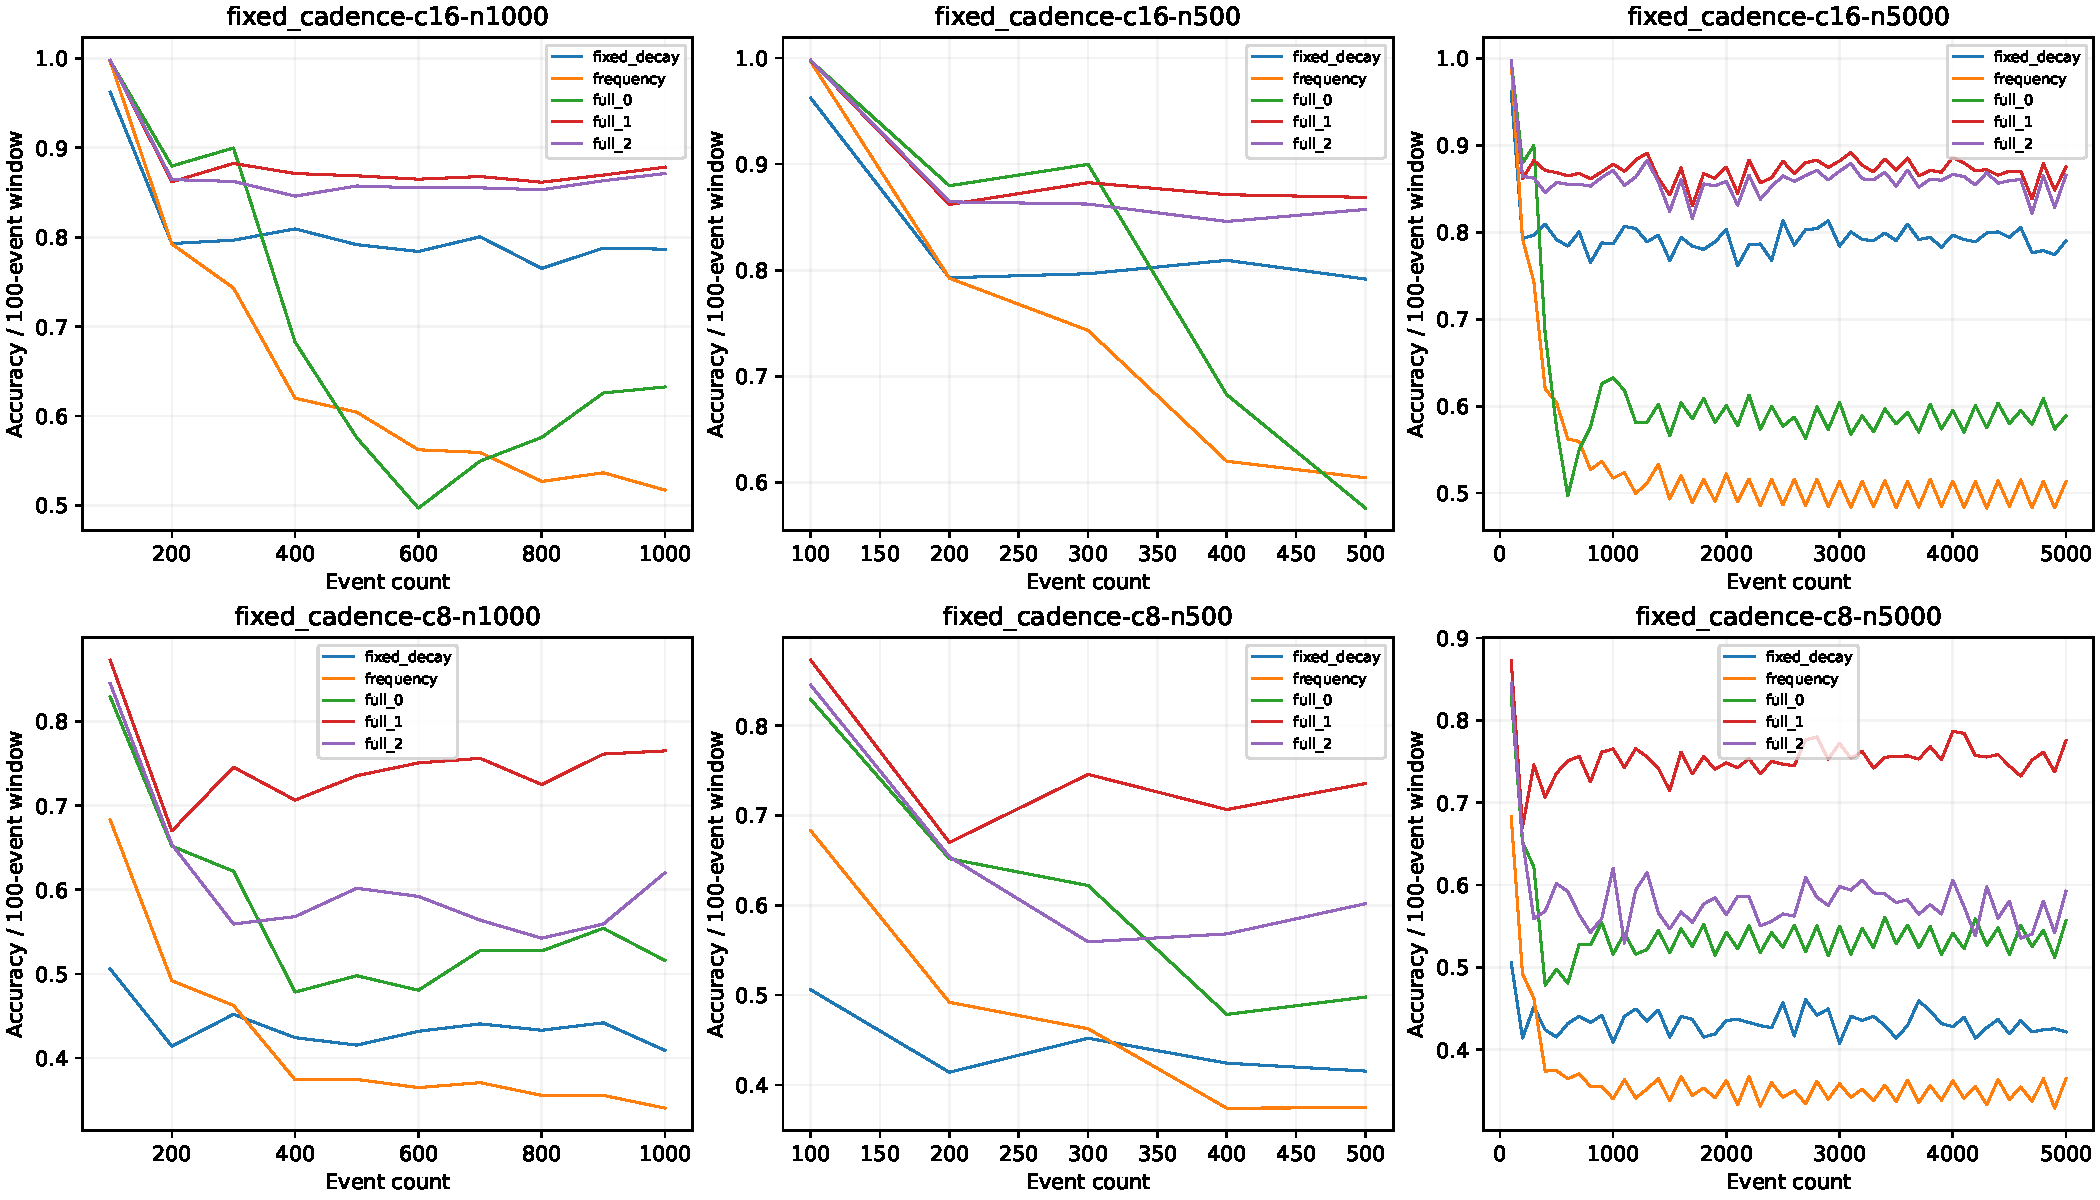
\includegraphics[width=\linewidth]{figures/long_horizon_performance.pdf}
\caption{All three predefined horizons and two capacities. Curves average 100-event window accuracy across frozen worlds and seeds. Shorter runs are exact prefixes; different panels must not be treated as independently generated environments.}\label{fig:long}
\end{figure}
\begin{figure}[p]\centering
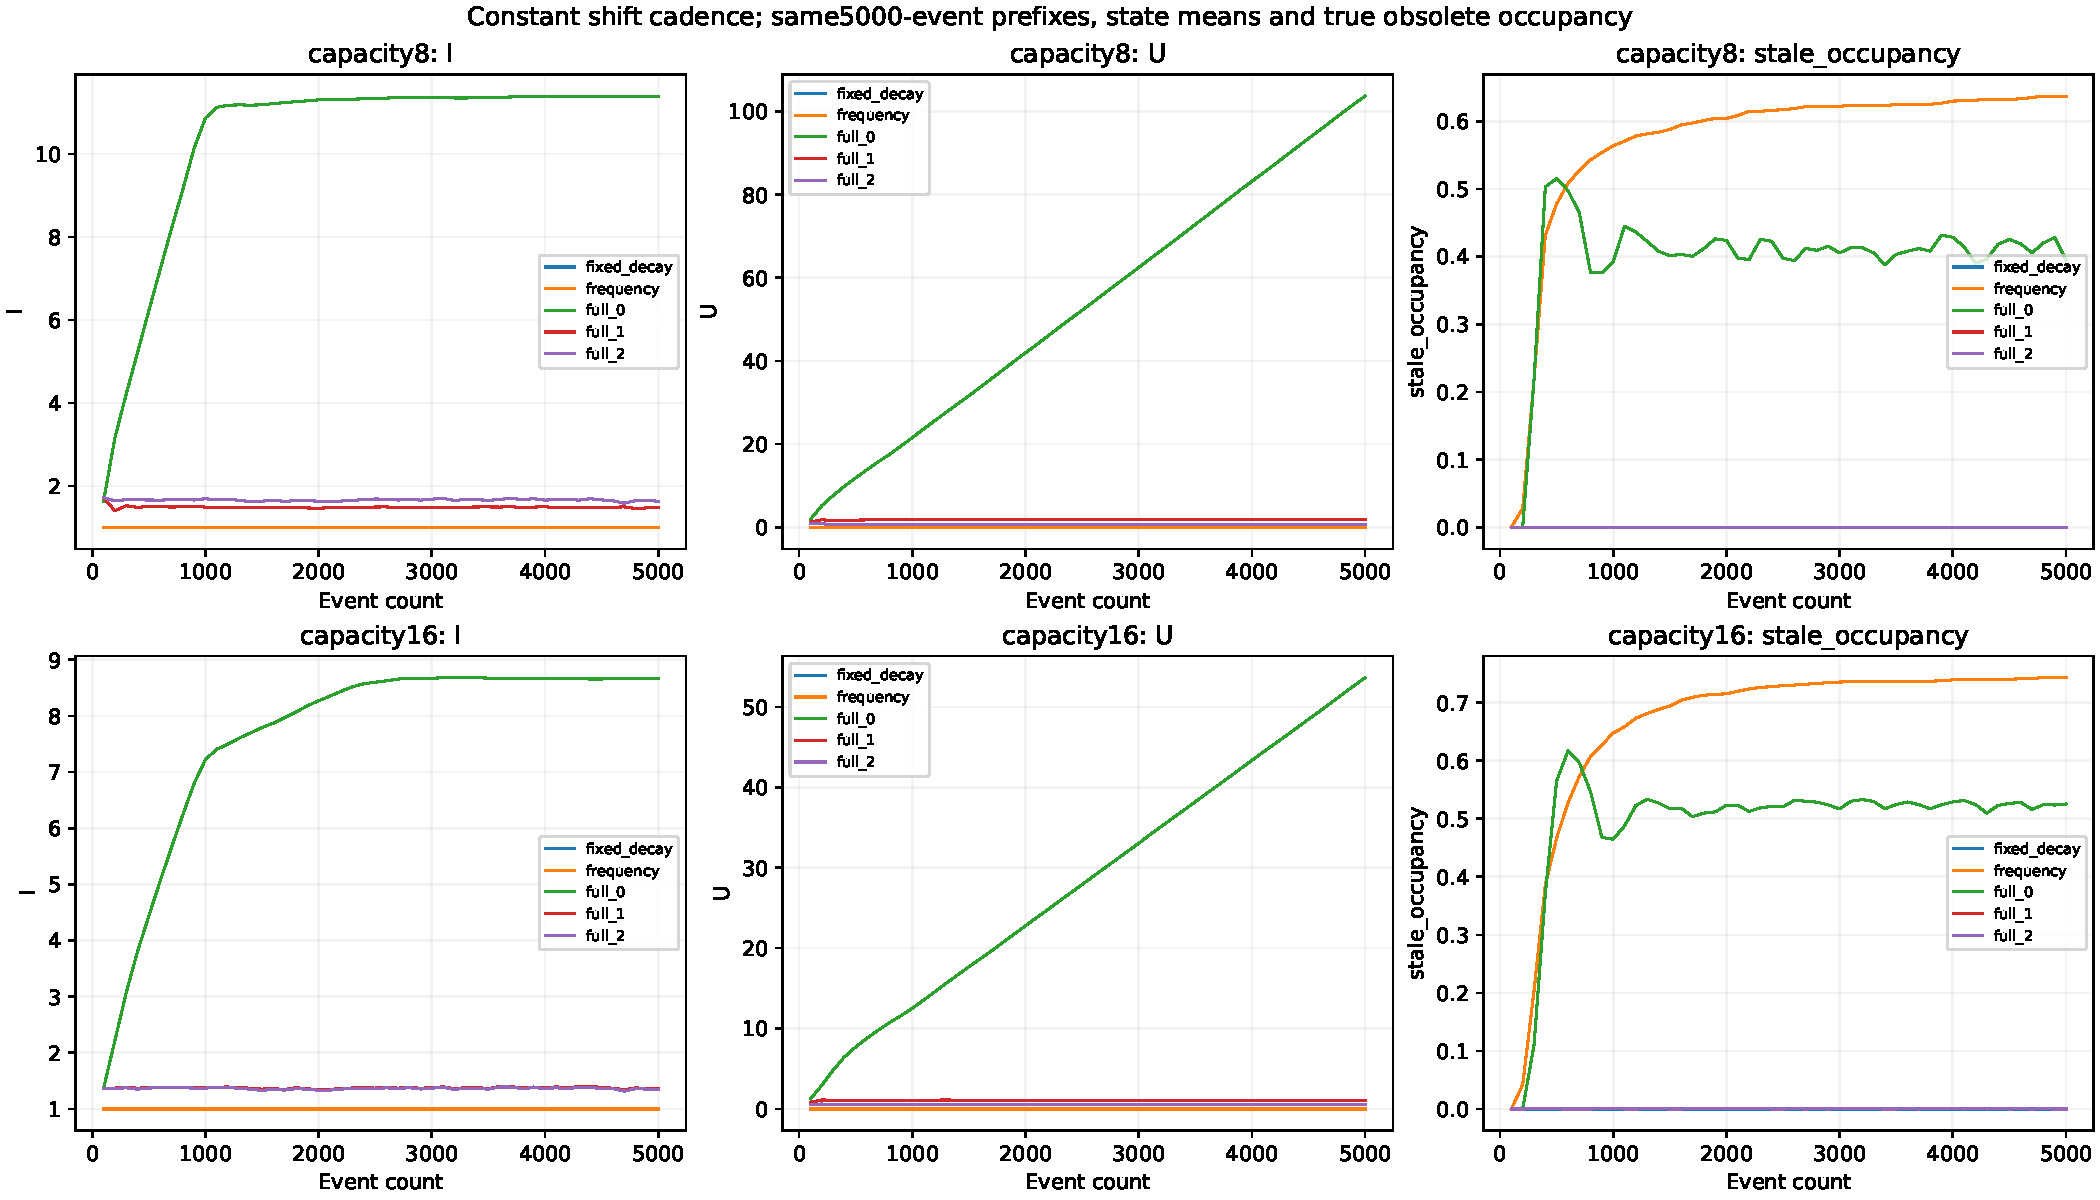
\includegraphics[width=\linewidth]{figures/long_horizon_states.pdf}
\caption{Long-horizon mean importance, usage, and obsolete-resident occupancy. Zero-strength usage growth follows the absence of usage decay. Fixed-policy state values are common implementation placeholders, not learned representations.}
\end{figure}

\subsection{Resource accounting}\label{app:resources}
The serial computational audit replays fixed environments separately from the parallel formal experiment. Policy time includes calls for state update, observation, retrieval, eviction, and feedback; it excludes trace serialization and language-model inference. Counts and Python object-graph estimates are saved in \texttt{serial\_computational\_audit.json}. These estimates include object bookkeeping and, in the full policy graph, retained lifetime logs; they are not isolated deployment RSS. A theoretical four-float64 state payload is 32 bytes per record, but common baseline records also allocate these fields. We therefore do not claim a measured 32-byte incremental cost or an efficiency advantage.

For 5,000-event stress trajectories at eight slots, strength one averages 39,959 item-state updates and 5,000 coefficient evaluations. Observed mean policy time is approximately 0.099 seconds versus 0.041 seconds for fixed decay, measured within four concurrent CPU workers. At sixteen slots these are approximately 0.131 and 0.050 seconds. They indicate extra work but are not clean speed benchmarks. Semantic addressing further requires resident embeddings and an encoder; offline embedding generation is excluded from policy-call time. All versions of the experiment retain growing auxiliary metadata or audit logs, so fixed content capacity must not be described as a strict total-memory guarantee.

\clearpage
\section{Complete Operating Points and State Traces}\label{app:operating}
\begin{figure}[h]
\centering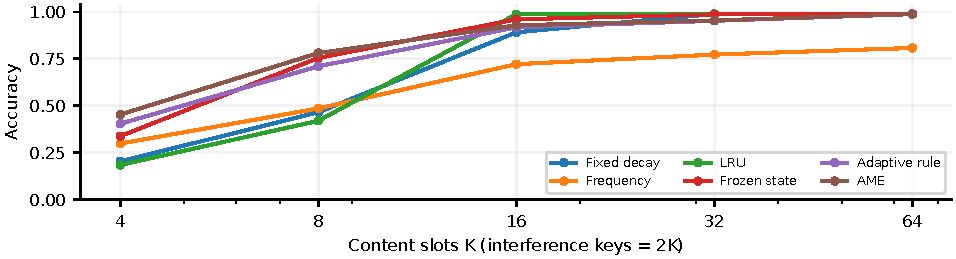
\includegraphics[width=.95\linewidth]{figures/capacity.pdf}
\caption{Capacity and interference jointly scale. All predefined budgets are shown; the larger-budget reversal rules out universal superiority. Complete replacement-control rows and intervals accompany the evidence files.}\label{fig:capacity}
\end{figure}
The main plot emphasizes eight-slot conditions for legibility; the following figure also includes both sixteen-slot conditions. The empirical nondominated envelope is computed only over this finite comparison set. Bootstrap frontier membership in the archive measures resampling stability, not a posterior probability of global optimality. All seven rates, including dominated points, remain in the tables.
\begin{figure}[h]\centering
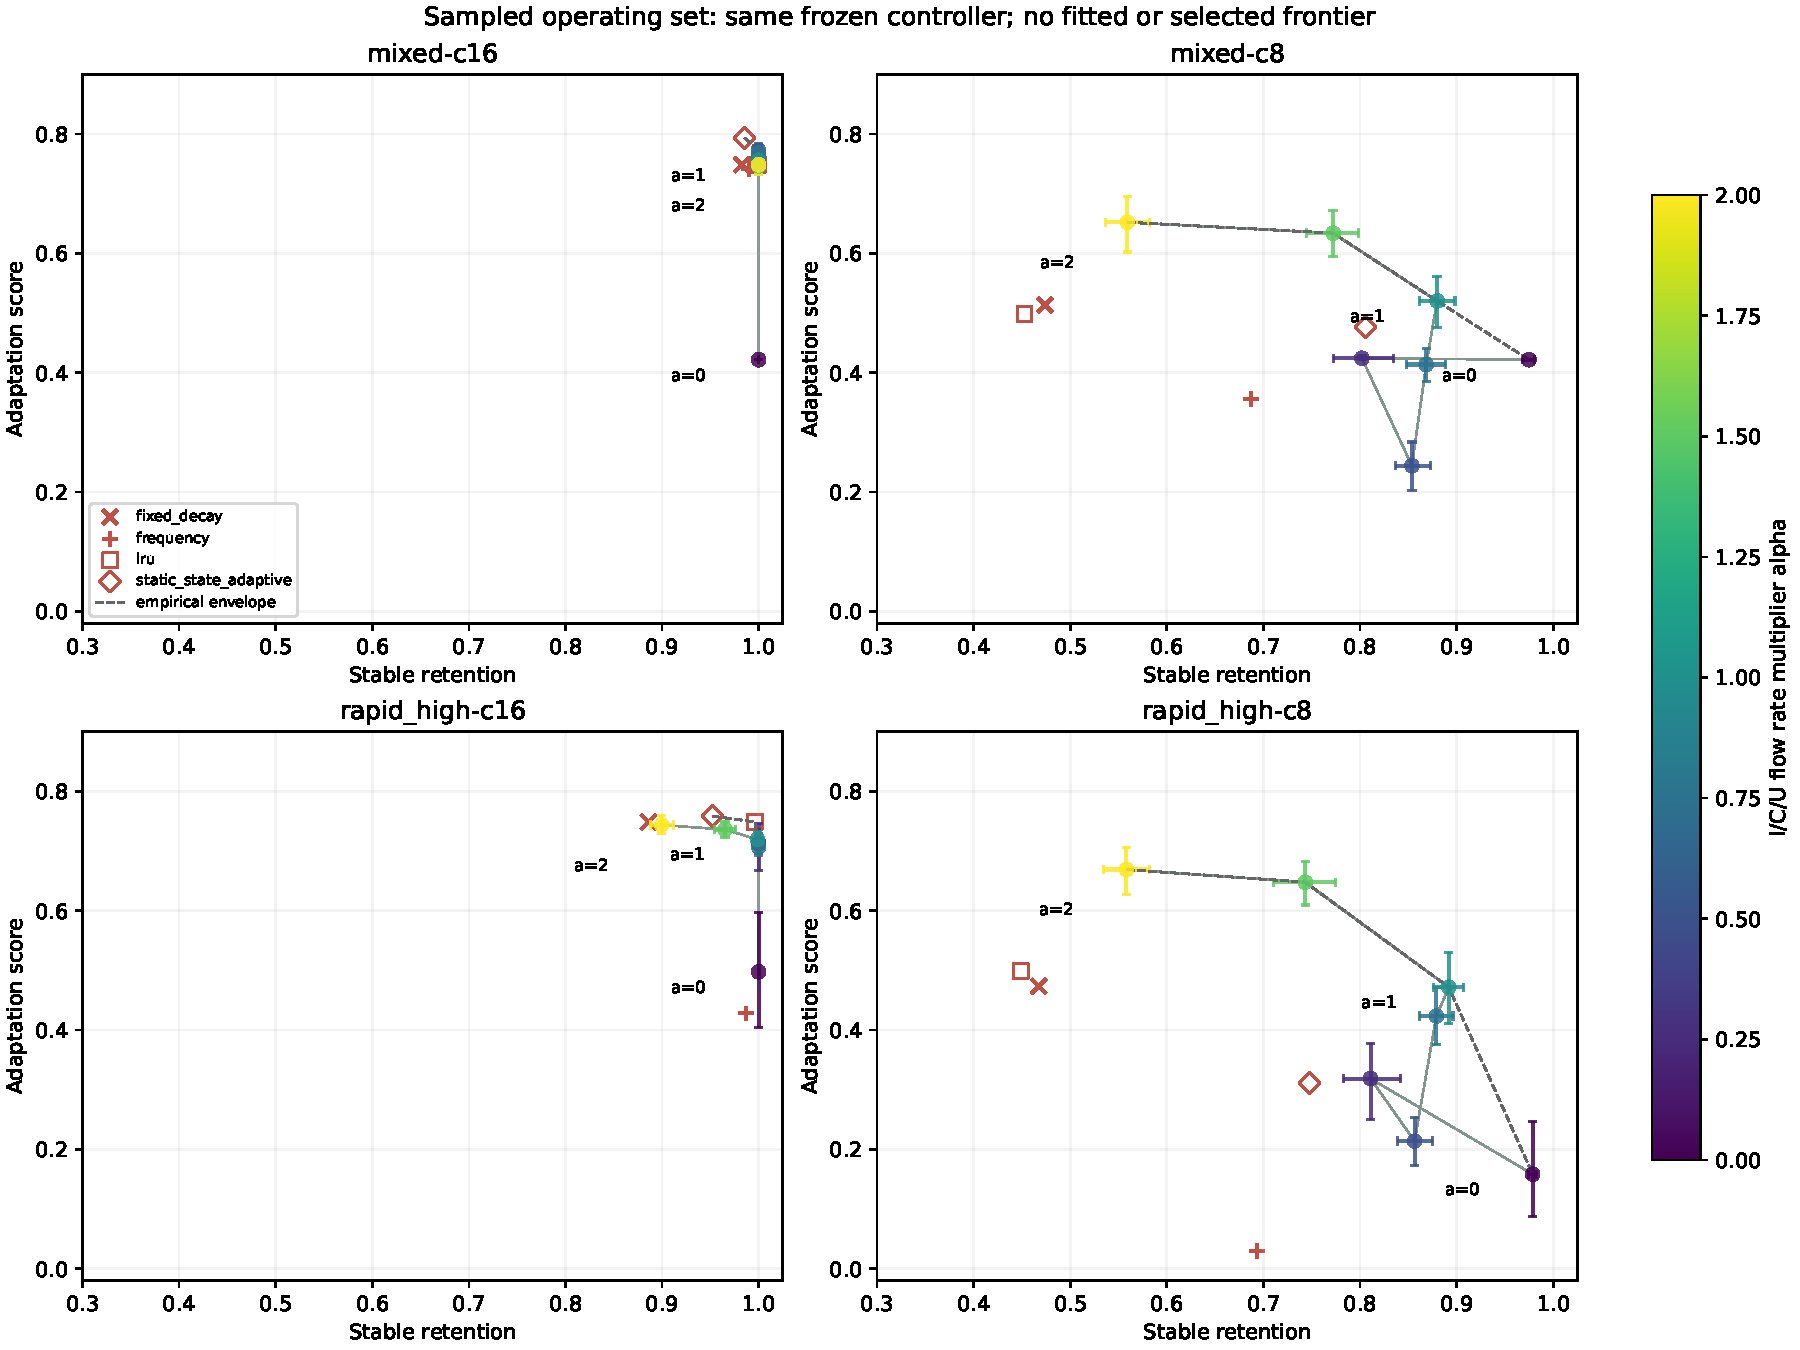
\includegraphics[width=.93\linewidth]{figures/all_operating_points.pdf}
\caption{All four C1 conditions. Capacity sixteen mixed demand saturates stable retention and has no rate pair with statistically supported opposing endpoint changes.}
\end{figure}
\clearpage
\begin{figure}[p]\centering
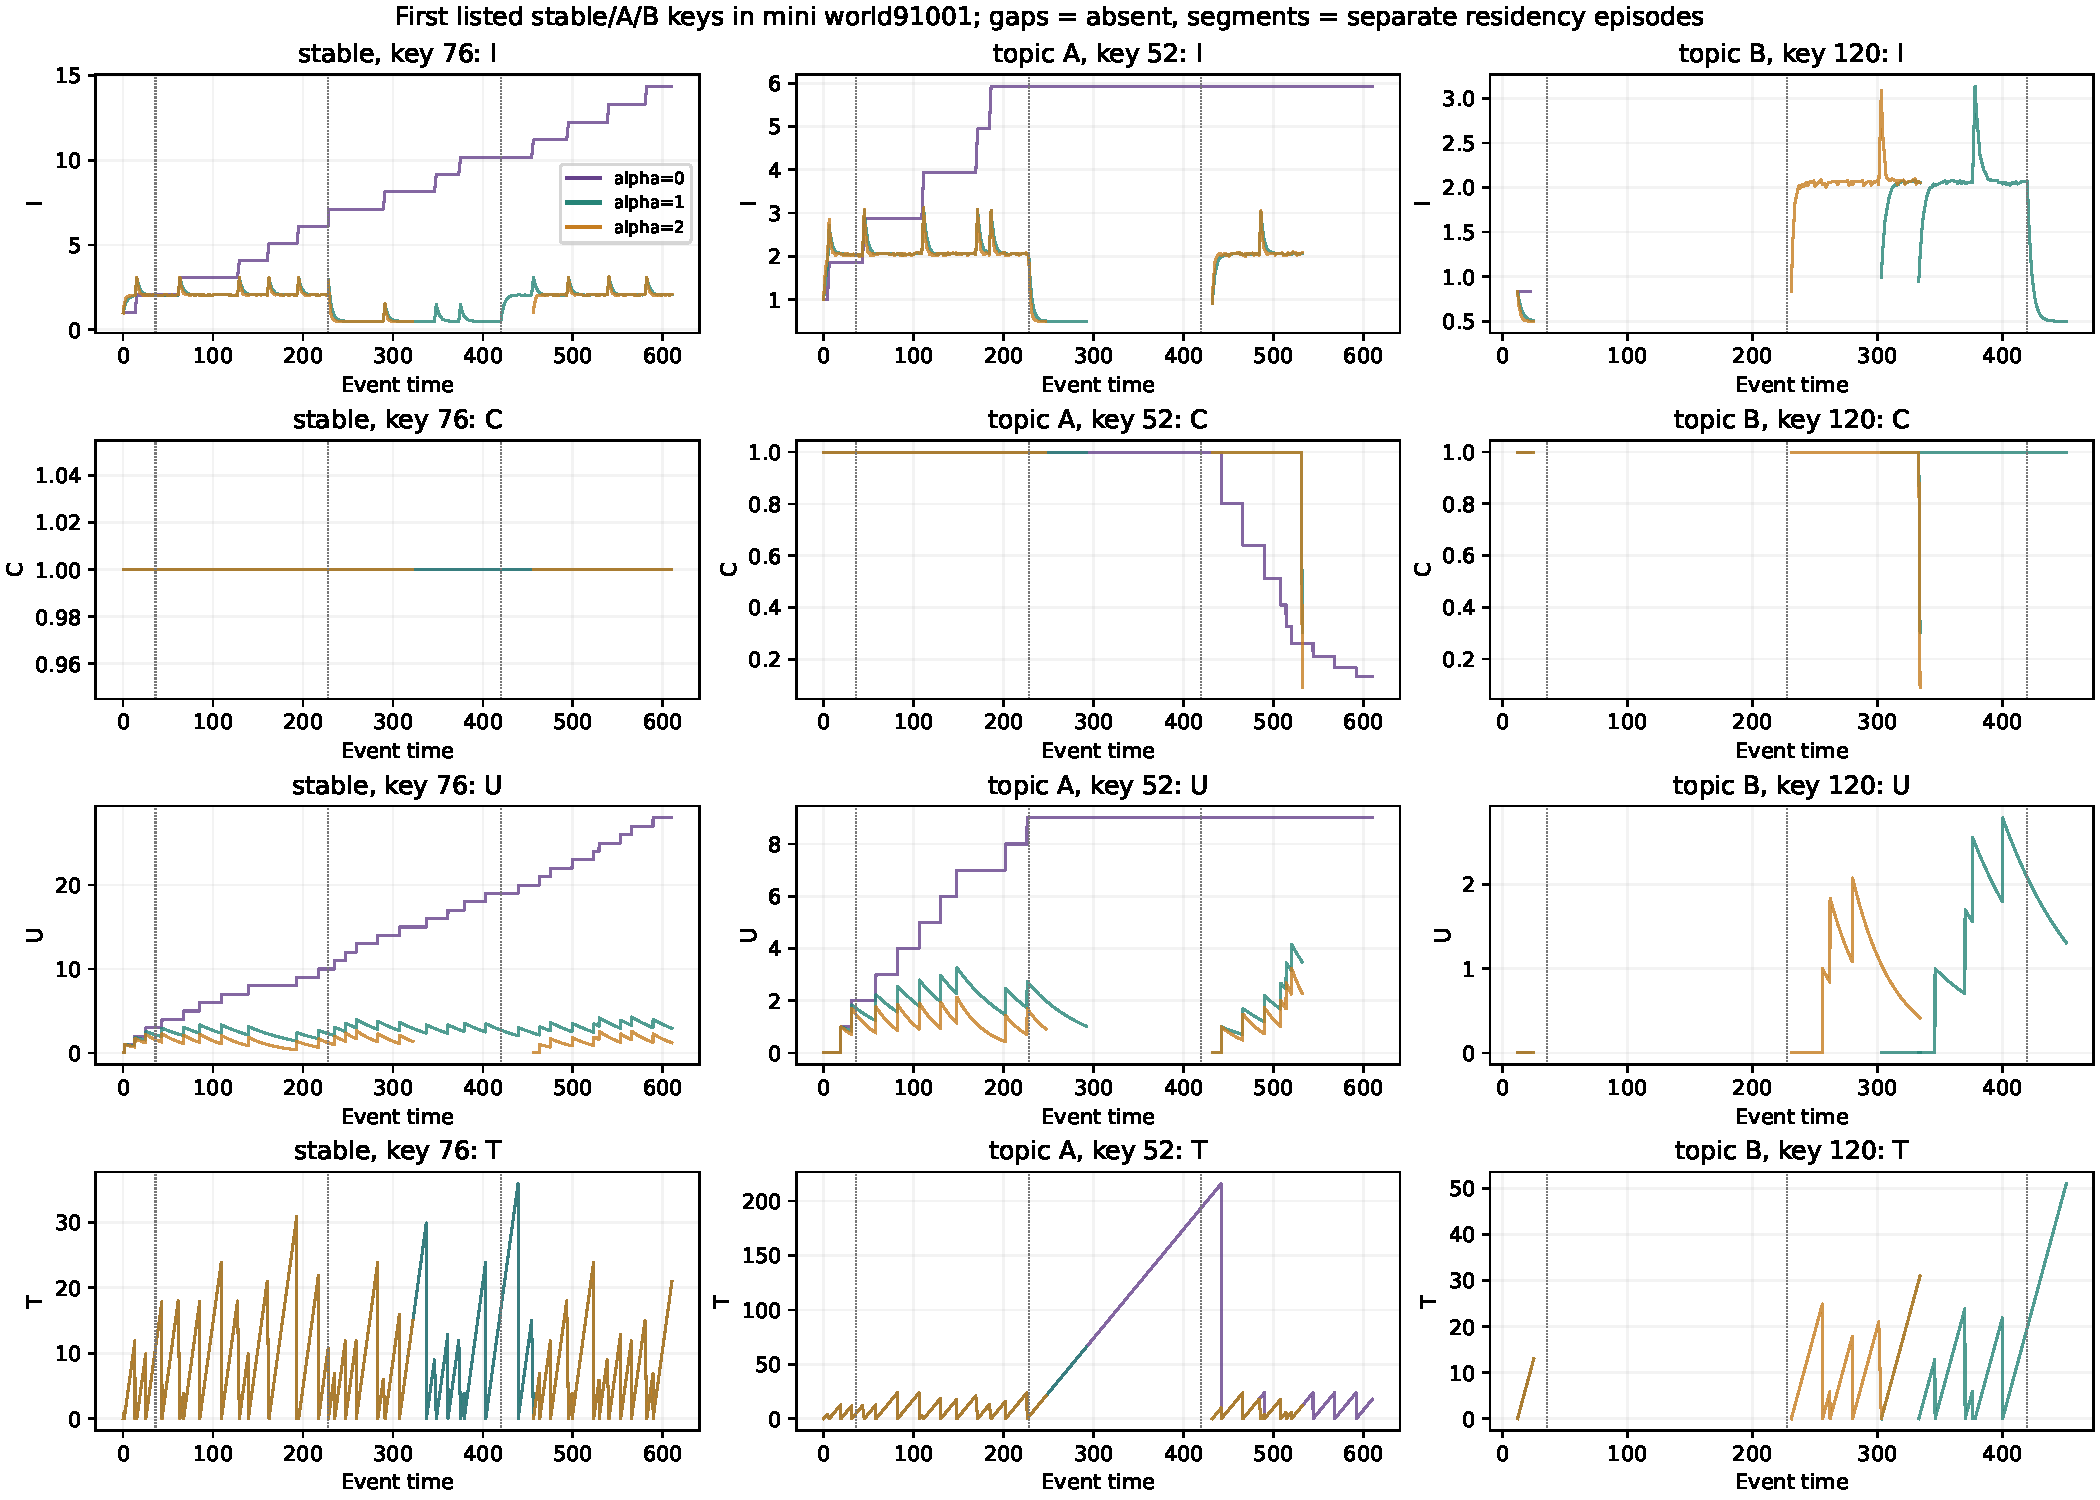
\includegraphics[width=\linewidth]{figures/selected_item_states.pdf}
\caption{Predefined first stable/A/B keys in mini world 91001 at strengths 0/1/2. All four states are shown. Missing segments denote absence from the resident store; separate residency episodes are not joined. Reappearance can therefore be distinguished from preservation of dormant content.}
\end{figure}
\clearpage
\section{Complete Numerical Results}\label{app:tables}
All rates and methods are retained. Main-text percentages are rounded from the frozen JSON summaries, not copied by hand into table cells. The evidence directory contains full world-level 95\% intervals and paired comparisons; the following compact tables show means for every condition. Their experimental batch identifiers are included only to connect each row to a frozen protocol, not as the main scientific organization of the paper. B1-A's full nine-cell attribution summary is also included in the evidence directory. Replacement-control rows do not imply successful lifetime-distribution matching.
\small
\begin{longtable}{llrrrr}\caption{B2: complete structured results (percentages; lag in queries).}\label{tab:B2}\\\toprule Condition & Policy & Acc. & Stale & Ret. & Lag\\\midrule\endfirsthead\toprule Condition & Policy & Acc. & Stale & Ret. & Lag\\\midrule\endhead
capacity4 & Fixed decay & 20.23 & 0.00 & 19.89 & 87.15\\
capacity4 & Frequency & 29.76 & 6.78 & 47.49 & 128.00\\
capacity4 & LRU & 18.33 & 0.00 & 18.03 & 101.96\\
capacity4 & Frozen state & 33.70 & 3.92 & 36.41 & 107.77\\
capacity4 & Replacement control$^{\dagger}$ & 26.88 & 0.61 & 34.78 & 122.90\\
capacity4 & Adaptive rule & 40.33 & 0.01 & 46.30 & 101.67\\
capacity4 & AME & 45.26 & 0.00 & 55.47 & 96.32\\
capacity8 & Fixed decay & 46.48 & 0.00 & 46.64 & 12.88\\
capacity8 & Frequency & 48.50 & 14.03 & 69.76 & 117.17\\
capacity8 & LRU & 41.91 & 0.00 & 42.10 & 17.29\\
capacity8 & Frozen state & 75.46 & 3.96 & 78.84 & 29.72\\
capacity8 & Replacement control$^{\dagger}$ & 54.93 & 1.81 & 74.84 & 103.77\\
capacity8 & Adaptive rule & 71.02 & 0.01 & 79.09 & 42.33\\
capacity8 & AME & 78.06 & 0.02 & 87.48 & 23.03\\
capacity16 & Fixed decay & 89.14 & 0.00 & 89.75 & 8.38\\
capacity16 & Frequency & 72.14 & 18.36 & 100.00 & 84.42\\
capacity16 & LRU & 98.81 & 0.00 & 99.74 & 8.23\\
capacity16 & Frozen state & 96.08 & 1.40 & 97.65 & 9.60\\
capacity16 & Replacement control$^{\dagger}$ & 77.74 & 4.35 & 99.70 & 71.71\\
capacity16 & Adaptive rule & 91.82 & 0.07 & 97.57 & 8.52\\
capacity16 & AME & 92.90 & 0.07 & 99.35 & 8.81\\
capacity32 & Fixed decay & 98.97 & 0.00 & 99.99 & 8.23\\
capacity32 & Frequency & 77.25 & 17.16 & 100.00 & 55.28\\
capacity32 & LRU & 98.99 & 0.00 & 100.00 & 8.23\\
capacity32 & Frozen state & 98.71 & 0.23 & 99.48 & 8.09\\
capacity32 & Replacement control$^{\dagger}$ & 91.31 & 3.77 & 100.00 & 21.81\\
capacity32 & Adaptive rule & 95.30 & 0.03 & 99.41 & 8.52\\
capacity32 & AME & 95.48 & 0.03 & 100.00 & 8.69\\
capacity64 & Fixed decay & 98.99 & 0.00 & 100.00 & 8.23\\
capacity64 & Frequency & 80.80 & 15.42 & 100.00 & 38.20\\
capacity64 & LRU & 98.99 & 0.00 & 100.00 & 8.23\\
capacity64 & Frozen state & 99.00 & 0.14 & 99.63 & 7.42\\
capacity64 & Replacement control$^{\dagger}$ & 97.36 & 1.00 & 100.00 & 10.03\\
capacity64 & Adaptive rule & 98.88 & 0.00 & 99.95 & 8.50\\
capacity64 & AME & 98.86 & 0.00 & 100.00 & 8.69\\
\bottomrule\end{longtable}
\begin{longtable}{llrrrr}\caption{B3: complete structured results (percentages; lag in queries).}\label{tab:B3}\\\toprule Condition & Policy & Acc. & Stale & Ret. & Lag\\\midrule\endfirsthead\toprule Condition & Policy & Acc. & Stale & Ret. & Lag\\\midrule\endhead
cyclic & Fixed decay & 44.18 & 0.00 & 46.09 & 18.29\\
cyclic & Frequency & 60.39 & 0.00 & 70.04 & 22.19\\
cyclic & LRU & 42.03 & 0.00 & 43.14 & 19.21\\
cyclic & Frozen state & 74.74 & 0.00 & 80.43 & 16.58\\
cyclic & Replacement control$^{\dagger}$ & 56.29 & 0.00 & 68.97 & 28.59\\
cyclic & Adaptive rule & 70.81 & 0.00 & 80.77 & 23.46\\
cyclic & AME & 78.66 & 0.00 & 86.76 & 16.65\\
\bottomrule\end{longtable}
\begin{longtable}{llrrrr}\caption{B4: complete structured results (percentages; lag in queries).}\label{tab:B4}\\\toprule Condition & Policy & Acc. & Stale & Ret. & Lag\\\midrule\endfirsthead\toprule Condition & Policy & Acc. & Stale & Ret. & Lag\\\midrule\endhead
clean & Fixed decay & 45.31 & 0.00 & 45.62 & 15.69\\
clean & Frequency & 49.01 & 11.96 & 68.48 & 29.45\\
clean & LRU & 43.14 & 0.00 & 43.84 & 17.33\\
clean & Frozen state & 65.91 & 3.60 & 75.00 & 22.88\\
clean & Replacement control$^{\dagger}$ & 51.74 & 2.01 & 67.26 & 28.10\\
clean & Adaptive rule & 71.42 & 0.02 & 83.33 & 19.60\\
clean & AME & 75.33 & 0.05 & 87.02 & 15.87\\
noise10 & Fixed decay & 45.31 & 0.00 & 45.62 & 15.69\\
noise10 & Frequency & 49.01 & 11.96 & 68.48 & 29.45\\
noise10 & LRU & 43.14 & 0.00 & 43.84 & 17.33\\
noise10 & Frozen state & 65.75 & 3.67 & 75.20 & 23.06\\
noise10 & Replacement control$^{\dagger}$ & 51.74 & 2.01 & 67.26 & 28.10\\
noise10 & Adaptive rule & 69.51 & 0.15 & 77.04 & 17.88\\
noise10 & AME & 74.75 & 0.05 & 83.81 & 15.24\\
noise25 & Fixed decay & 45.31 & 0.00 & 45.62 & 15.69\\
noise25 & Frequency & 49.01 & 11.96 & 68.48 & 29.45\\
noise25 & LRU & 43.14 & 0.00 & 43.84 & 17.33\\
noise25 & Frozen state & 65.34 & 3.79 & 73.90 & 22.31\\
noise25 & Replacement control$^{\dagger}$ & 51.74 & 2.01 & 67.26 & 28.10\\
noise25 & Adaptive rule & 65.21 & 0.07 & 65.71 & 14.27\\
noise25 & AME & 72.10 & 0.07 & 76.32 & 13.60\\
noise50 & Fixed decay & 45.31 & 0.00 & 45.62 & 15.69\\
noise50 & Frequency & 49.01 & 11.96 & 68.48 & 29.45\\
noise50 & LRU & 43.14 & 0.00 & 43.84 & 17.33\\
noise50 & Frozen state & 65.08 & 3.83 & 73.84 & 22.69\\
noise50 & Replacement control$^{\dagger}$ & 51.74 & 2.01 & 67.26 & 28.10\\
noise50 & Adaptive rule & 60.66 & 0.07 & 50.65 & 12.04\\
noise50 & AME & 64.59 & 0.09 & 57.77 & 12.24\\
misleading\_importance & Fixed decay & 45.31 & 0.00 & 45.62 & 15.69\\
misleading\_importance & Frequency & 49.01 & 11.96 & 68.48 & 29.45\\
misleading\_importance & LRU & 43.14 & 0.00 & 43.84 & 17.33\\
misleading\_importance & Frozen state & 67.49 & 5.24 & 85.37 & 26.47\\
misleading\_importance & Replacement control$^{\dagger}$ & 51.74 & 2.01 & 67.26 & 28.10\\
misleading\_importance & Adaptive rule & 48.03 & 0.00 & 78.82 & 29.79\\
misleading\_importance & AME & 50.33 & 0.01 & 80.92 & 30.17\\
\bottomrule\end{longtable}
\begin{longtable}{llrrrr}\caption{B5: complete structured results (percentages; lag in queries).}\label{tab:B5}\\\toprule Condition & Policy & Acc. & Stale & Ret. & Lag\\\midrule\endfirsthead\toprule Condition & Policy & Acc. & Stale & Ret. & Lag\\\midrule\endhead
version\_update & Fixed decay & 45.05 & 0.00 & 45.92 & 17.92\\
version\_update & Frequency & 50.65 & 11.31 & 72.80 & 29.82\\
version\_update & LRU & 43.42 & 0.00 & 44.44 & 17.04\\
version\_update & Frozen state & 66.59 & 3.41 & 73.94 & 20.92\\
version\_update & Replacement control$^{\dagger}$ & 51.40 & 2.39 & 66.62 & 26.96\\
version\_update & Adaptive rule & 69.31 & 0.09 & 82.42 & 20.98\\
version\_update & AME & 74.42 & 0.09 & 87.86 & 16.31\\
\bottomrule\end{longtable}
\begin{longtable}{llrrrr}\caption{B6: complete structured results (percentages; lag in queries).}\label{tab:B6}\\\toprule Condition & Policy & Acc. & Stale & Ret. & Lag\\\midrule\endfirsthead\toprule Condition & Policy & Acc. & Stale & Ret. & Lag\\\midrule\endhead
rapid\_high & Fixed decay & 44.64 & 0.00 & 45.36 & 17.29\\
rapid\_high & Frequency & 50.46 & 11.48 & 70.69 & 29.42\\
rapid\_high & LRU & 42.69 & 0.00 & 43.40 & 19.19\\
rapid\_high & Frozen state & 66.89 & 3.05 & 73.80 & 20.74\\
rapid\_high & Replacement control$^{\dagger}$ & 51.95 & 1.81 & 66.71 & 27.51\\
rapid\_high & Adaptive rule & 68.51 & 0.09 & 79.04 & 19.62\\
rapid\_high & AME & 75.02 & 0.07 & 88.25 & 15.53\\
rapid\_high & No importance & 67.14 & 0.02 & 91.70 & 26.72\\
rapid\_high & No consistency & 70.20 & 8.76 & 86.88 & 16.66\\
rapid\_high & No usage & 57.91 & 0.11 & 48.51 & 12.85\\
rapid\_high & No temporal state & 74.17 & 0.09 & 88.34 & 17.46\\
\bottomrule\end{longtable}
\begin{longtable}{llrrrr}\caption{B7: complete structured results (percentages; lag in queries).}\label{tab:B7}\\\toprule Condition & Policy & Acc. & Stale & Ret. & Lag\\\midrule\endfirsthead\toprule Condition & Policy & Acc. & Stale & Ret. & Lag\\\midrule\endhead
rapid\_high & Fixed decay & 44.94 & 0.00 & 46.44 & 17.06\\
rapid\_high & Frequency & 49.83 & 11.48 & 69.59 & 28.60\\
rapid\_high & LRU & 43.08 & 0.00 & 44.70 & 18.71\\
rapid\_high & Frozen state & 66.44 & 3.88 & 75.33 & 20.81\\
rapid\_high & Replacement control$^{\dagger}$ & 50.92 & 1.98 & 65.81 & 28.31\\
rapid\_high & Adaptive rule & 69.18 & 0.09 & 83.33 & 21.48\\
rapid\_high & AME & 74.80 & 0.09 & 87.27 & 16.01\\
rapid\_high & event\_only & 67.26 & 14.74 & 98.31 & 26.38\\
rapid\_high & discrete\_euler & 74.18 & 0.09 & 86.92 & 17.05\\
rapid\_high & query\_conditioned & 72.49 & 0.08 & 85.14 & 19.88\\
\bottomrule\end{longtable}
\begin{longtable}{llrrr}\caption{Fixed-subset language transfer. Quality is binary judged correctness for conversational QA and normalized rubric quality for NFCats; these scales must not be pooled.}\label{tab:language}\\\toprule Dataset & Policy & Quality & 95\% CI & Evidence hit\\\midrule\endfirsthead\toprule Dataset & Policy & Quality & 95\% CI & Evidence hit\\\midrule\endhead
LoCoMo & Fixed decay & 0.033 & [0.000,0.100] & 0.067\\
LoCoMo & Frequency & 0.100 & [0.017,0.233] & 0.094\\
LoCoMo & LRU & 0.050 & [0.000,0.133] & 0.067\\
LoCoMo & Frozen state & 0.011 & [0.000,0.033] & 0.061\\
LoCoMo & Replacement control$^{\dagger}$ & 0.044 & [0.000,0.122] & 0.089\\
LoCoMo & Adaptive rule & 0.094 & [0.000,0.211] & 0.094\\
LoCoMo & AME & 0.111 & [0.017,0.222] & 0.111\\
LongMemEval & Fixed decay & 0.153 & [0.028,0.306] & 0.167\\
LongMemEval & Frequency & 0.069 & [0.028,0.125] & 0.736\\
LongMemEval & LRU & 0.139 & [0.014,0.278] & 0.208\\
LongMemEval & Frozen state & 0.111 & [0.028,0.208] & 0.528\\
LongMemEval & Replacement control$^{\dagger}$ & 0.250 & [0.097,0.417] & 0.278\\
LongMemEval & Adaptive rule & 0.083 & [0.000,0.208] & 0.264\\
LongMemEval & AME & 0.042 & [0.000,0.111] & 0.306\\
NFCats & Fixed decay & 0.733 & [0.583,0.854] & --\\
NFCats & Frequency & 0.736 & [0.618,0.840] & --\\
NFCats & LRU & 0.740 & [0.604,0.865] & --\\
NFCats & Frozen state & 0.642 & [0.507,0.767] & --\\
NFCats & Replacement control$^{\dagger}$ & 0.743 & [0.611,0.858] & --\\
NFCats & Adaptive rule & 0.660 & [0.517,0.788] & --\\
NFCats & AME & 0.740 & [0.632,0.840] & --\\
\bottomrule\end{longtable}
\begin{longtable}{llrrrr}\caption{C1: all frozen operating points. Percentages except adaptation score.}\label{tab:C1}\\\toprule Condition & Policy & Acc. & Stale & Ret. & Adapt.\\\midrule\endfirsthead\toprule Condition & Policy & Acc. & Stale & Ret. & Adapt.\\\midrule\endhead
mixed-c16 & fixed\_decay & 95.29 & 0.00 & 98.26 & 0.749\\
mixed-c16 & frequency & 93.99 & 0.00 & 99.03 & 0.742\\
mixed-c16 & lru & 96.16 & 0.00 & 99.91 & 0.749\\
mixed-c16 & static\_state\_adaptive & 96.70 & 0.00 & 98.54 & 0.794\\
mixed-c16 & full\_0 & 83.33 & 0.00 & 100.00 & 0.422\\
mixed-c16 & full\_0.25 & 97.09 & 0.00 & 100.00 & 0.763\\
mixed-c16 & full\_0.5 & 96.73 & 0.00 & 100.00 & 0.772\\
mixed-c16 & full\_0.75 & 96.65 & 0.00 & 100.00 & 0.768\\
mixed-c16 & full\_1 & 96.44 & 0.00 & 100.00 & 0.756\\
mixed-c16 & full\_1.5 & 96.15 & 0.00 & 100.00 & 0.747\\
mixed-c16 & full\_2 & 96.20 & 0.00 & 100.00 & 0.749\\
mixed-c8 & fixed\_decay & 45.96 & 0.00 & 47.40 & 0.514\\
mixed-c8 & frequency & 61.24 & 0.00 & 68.69 & 0.356\\
mixed-c8 & lru & 43.90 & 0.00 & 45.27 & 0.499\\
mixed-c8 & static\_state\_adaptive & 75.00 & 0.00 & 80.57 & 0.477\\
mixed-c8 & full\_0 & 81.26 & 0.00 & 97.50 & 0.422\\
mixed-c8 & full\_0.25 & 75.56 & 0.00 & 80.19 & 0.424\\
mixed-c8 & full\_0.5 & 73.87 & 0.00 & 85.37 & 0.244\\
mixed-c8 & full\_0.75 & 78.39 & 0.00 & 86.85 & 0.414\\
mixed-c8 & full\_1 & 80.82 & 0.00 & 87.98 & 0.520\\
mixed-c8 & full\_1.5 & 78.33 & 0.00 & 77.21 & 0.634\\
mixed-c8 & full\_2 & 68.69 & 0.00 & 55.92 & 0.652\\
rapid\_high-c16 & fixed\_decay & 85.92 & 0.00 & 88.59 & 0.749\\
rapid\_high-c16 & frequency & 75.81 & 16.50 & 98.68 & 0.428\\
rapid\_high-c16 & lru & 95.92 & 0.00 & 99.61 & 0.749\\
rapid\_high-c16 & static\_state\_adaptive & 91.29 & 2.11 & 95.23 & 0.758\\
rapid\_high-c16 & full\_0 & 76.92 & 19.44 & 100.00 & 0.497\\
rapid\_high-c16 & full\_0.25 & 89.73 & 0.77 & 100.00 & 0.713\\
rapid\_high-c16 & full\_0.5 & 92.66 & 0.14 & 100.00 & 0.712\\
rapid\_high-c16 & full\_0.75 & 94.06 & 0.03 & 100.00 & 0.707\\
rapid\_high-c16 & full\_1 & 93.40 & 0.02 & 99.87 & 0.719\\
rapid\_high-c16 & full\_1.5 & 92.39 & 0.02 & 96.53 & 0.736\\
rapid\_high-c16 & full\_2 & 90.44 & 0.02 & 89.96 & 0.743\\
rapid\_high-c8 & fixed\_decay & 45.10 & 0.00 & 46.74 & 0.473\\
rapid\_high-c8 & frequency & 49.50 & 11.17 & 69.37 & 0.029\\
rapid\_high-c8 & lru & 43.36 & 0.00 & 44.88 & 0.499\\
rapid\_high-c8 & static\_state\_adaptive & 66.13 & 3.56 & 74.77 & 0.311\\
rapid\_high-c8 & full\_0 & 66.63 & 14.79 & 97.87 & 0.158\\
rapid\_high-c8 & full\_0.25 & 65.78 & 0.69 & 81.09 & 0.318\\
rapid\_high-c8 & full\_0.5 & 70.80 & 0.13 & 85.65 & 0.214\\
rapid\_high-c8 & full\_0.75 & 74.88 & 0.07 & 87.91 & 0.423\\
rapid\_high-c8 & full\_1 & 76.28 & 0.10 & 89.19 & 0.472\\
rapid\_high-c8 & full\_1.5 & 72.43 & 0.05 & 74.33 & 0.648\\
rapid\_high-c8 & full\_2 & 63.99 & 0.06 & 55.82 & 0.669\\
\bottomrule\end{longtable}
\begin{longtable}{llrrrr}\caption{C2: all frozen operating points. Percentages except adaptation score.}\label{tab:C2}\\\toprule Condition & Policy & Acc. & Stale & Ret. & Adapt.\\\midrule\endfirsthead\toprule Condition & Policy & Acc. & Stale & Ret. & Adapt.\\\midrule\endhead
mixed-c16 & fixed\_decay & 95.27 & 0.00 & 98.83 & 0.748\\
mixed-c16 & frequency & 93.41 & 0.00 & 99.32 & 0.717\\
mixed-c16 & lru & 96.01 & 0.00 & 99.96 & 0.748\\
mixed-c16 & static\_state\_adaptive & 96.28 & 0.00 & 98.37 & 0.794\\
mixed-c16 & full\_0 & 83.33 & 0.00 & 100.00 & 0.422\\
mixed-c16 & full\_0.25 & 96.85 & 0.00 & 100.00 & 0.763\\
mixed-c16 & full\_0.5 & 96.81 & 0.00 & 100.00 & 0.769\\
mixed-c16 & full\_0.75 & 96.43 & 0.00 & 100.00 & 0.759\\
mixed-c16 & full\_1 & 96.20 & 0.00 & 100.00 & 0.754\\
mixed-c16 & full\_1.5 & 95.92 & 0.00 & 99.83 & 0.748\\
mixed-c16 & full\_2 & 95.96 & 0.00 & 99.87 & 0.748\\
mixed-c16 & I\_0 & 83.33 & 0.00 & 100.00 & 0.422\\
mixed-c16 & I\_0.25 & 96.85 & 0.00 & 100.00 & 0.763\\
mixed-c16 & I\_0.5 & 97.20 & 0.00 & 100.00 & 0.769\\
mixed-c16 & I\_0.75 & 97.58 & 0.00 & 100.00 & 0.784\\
mixed-c16 & I\_1 & 97.68 & 0.00 & 100.00 & 0.786\\
mixed-c16 & I\_1.5 & 97.89 & 0.00 & 100.00 & 0.793\\
mixed-c16 & I\_2 & 97.92 & 0.00 & 100.00 & 0.794\\
mixed-c16 & C\_0 & 83.33 & 0.00 & 100.00 & 0.422\\
mixed-c16 & C\_0.25 & 83.33 & 0.00 & 100.00 & 0.422\\
mixed-c16 & C\_0.5 & 83.33 & 0.00 & 100.00 & 0.422\\
mixed-c16 & C\_0.75 & 83.33 & 0.00 & 100.00 & 0.422\\
mixed-c16 & C\_1 & 83.33 & 0.00 & 100.00 & 0.422\\
mixed-c16 & C\_1.5 & 83.33 & 0.00 & 100.00 & 0.422\\
mixed-c16 & C\_2 & 83.33 & 0.00 & 100.00 & 0.422\\
mixed-c16 & U\_0 & 83.33 & 0.00 & 100.00 & 0.422\\
mixed-c16 & U\_0.25 & 83.33 & 0.00 & 100.00 & 0.422\\
mixed-c16 & U\_0.5 & 83.33 & 0.00 & 100.00 & 0.422\\
mixed-c16 & U\_0.75 & 83.33 & 0.00 & 100.00 & 0.422\\
mixed-c16 & U\_1 & 83.33 & 0.00 & 100.00 & 0.422\\
mixed-c16 & U\_1.5 & 83.33 & 0.00 & 100.00 & 0.422\\
mixed-c16 & U\_2 & 83.33 & 0.00 & 100.00 & 0.422\\
mixed-c8 & fixed\_decay & 45.72 & 0.00 & 46.48 & 0.551\\
mixed-c8 & frequency & 61.96 & 0.00 & 71.77 & 0.362\\
mixed-c8 & lru & 43.97 & 0.00 & 45.62 & 0.531\\
mixed-c8 & static\_state\_adaptive & 74.39 & 0.00 & 79.44 & 0.473\\
mixed-c8 & full\_0 & 80.97 & 0.00 & 96.79 & 0.422\\
mixed-c8 & full\_0.25 & 74.65 & 0.00 & 78.52 & 0.422\\
mixed-c8 & full\_0.5 & 72.36 & 0.00 & 83.65 & 0.268\\
mixed-c8 & full\_0.75 & 78.31 & 0.00 & 86.63 & 0.428\\
mixed-c8 & full\_1 & 79.64 & 0.00 & 86.36 & 0.486\\
mixed-c8 & full\_1.5 & 76.62 & 0.00 & 73.80 & 0.624\\
mixed-c8 & full\_2 & 68.72 & 0.00 & 53.08 & 0.683\\
mixed-c8 & I\_0 & 80.97 & 0.00 & 96.79 & 0.422\\
mixed-c8 & I\_0.25 & 74.65 & 0.00 & 78.52 & 0.422\\
mixed-c8 & I\_0.5 & 73.42 & 0.00 & 77.31 & 0.422\\
mixed-c8 & I\_0.75 & 73.30 & 0.00 & 75.43 & 0.422\\
mixed-c8 & I\_1 & 73.47 & 0.00 & 75.39 & 0.422\\
mixed-c8 & I\_1.5 & 73.20 & 0.00 & 75.39 & 0.422\\
mixed-c8 & I\_2 & 73.23 & 0.00 & 75.39 & 0.422\\
mixed-c8 & C\_0 & 80.97 & 0.00 & 96.79 & 0.422\\
mixed-c8 & C\_0.25 & 80.97 & 0.00 & 96.79 & 0.422\\
mixed-c8 & C\_0.5 & 80.97 & 0.00 & 96.79 & 0.422\\
mixed-c8 & C\_0.75 & 80.97 & 0.00 & 96.79 & 0.422\\
mixed-c8 & C\_1 & 80.97 & 0.00 & 96.79 & 0.422\\
mixed-c8 & C\_1.5 & 80.97 & 0.00 & 96.79 & 0.422\\
mixed-c8 & C\_2 & 80.97 & 0.00 & 96.79 & 0.422\\
mixed-c8 & U\_0 & 80.97 & 0.00 & 96.79 & 0.422\\
mixed-c8 & U\_0.25 & 80.97 & 0.00 & 96.79 & 0.422\\
mixed-c8 & U\_0.5 & 80.97 & 0.00 & 96.79 & 0.422\\
mixed-c8 & U\_0.75 & 80.93 & 0.00 & 96.79 & 0.422\\
mixed-c8 & U\_1 & 80.93 & 0.00 & 96.79 & 0.422\\
mixed-c8 & U\_1.5 & 80.93 & 0.00 & 96.79 & 0.422\\
mixed-c8 & U\_2 & 80.96 & 0.00 & 96.79 & 0.423\\
rapid\_high-c16 & fixed\_decay & 85.85 & 0.00 & 88.59 & 0.748\\
rapid\_high-c16 & frequency & 76.19 & 16.79 & 98.97 & 0.426\\
rapid\_high-c16 & lru & 95.55 & 0.00 & 99.31 & 0.748\\
rapid\_high-c16 & static\_state\_adaptive & 90.76 & 2.26 & 94.72 & 0.742\\
rapid\_high-c16 & full\_0 & 77.11 & 18.99 & 100.00 & 0.538\\
rapid\_high-c16 & full\_0.25 & 89.23 & 0.93 & 100.00 & 0.688\\
rapid\_high-c16 & full\_0.5 & 92.13 & 0.24 & 100.00 & 0.707\\
rapid\_high-c16 & full\_0.75 & 94.06 & 0.00 & 100.00 & 0.707\\
rapid\_high-c16 & full\_1 & 92.89 & 0.03 & 99.57 & 0.712\\
rapid\_high-c16 & full\_1.5 & 91.64 & 0.04 & 96.48 & 0.731\\
rapid\_high-c16 & full\_2 & 90.44 & 0.00 & 90.91 & 0.736\\
rapid\_high-c16 & I\_0 & 77.11 & 18.99 & 100.00 & 0.538\\
rapid\_high-c16 & I\_0.25 & 81.90 & 12.64 & 100.00 & 0.688\\
rapid\_high-c16 & I\_0.5 & 82.95 & 12.79 & 100.00 & 0.735\\
rapid\_high-c16 & I\_0.75 & 83.20 & 13.00 & 100.00 & 0.755\\
rapid\_high-c16 & I\_1 & 83.76 & 12.50 & 100.00 & 0.769\\
rapid\_high-c16 & I\_1.5 & 84.21 & 12.41 & 100.00 & 0.779\\
rapid\_high-c16 & I\_2 & 84.21 & 12.41 & 100.00 & 0.779\\
rapid\_high-c16 & C\_0 & 77.11 & 18.99 & 100.00 & 0.538\\
rapid\_high-c16 & C\_0.25 & 83.12 & 11.82 & 100.00 & 0.614\\
rapid\_high-c16 & C\_0.5 & 83.37 & 11.78 & 100.00 & 0.609\\
rapid\_high-c16 & C\_0.75 & 83.69 & 11.94 & 100.00 & 0.609\\
rapid\_high-c16 & C\_1 & 83.70 & 11.94 & 100.00 & 0.609\\
rapid\_high-c16 & C\_1.5 & 83.70 & 11.94 & 100.00 & 0.609\\
rapid\_high-c16 & C\_2 & 83.70 & 11.94 & 100.00 & 0.609\\
rapid\_high-c16 & U\_0 & 77.11 & 18.99 & 100.00 & 0.538\\
rapid\_high-c16 & U\_0.25 & 77.27 & 18.80 & 100.00 & 0.538\\
rapid\_high-c16 & U\_0.5 & 78.30 & 17.72 & 100.00 & 0.538\\
rapid\_high-c16 & U\_0.75 & 80.16 & 15.79 & 100.00 & 0.553\\
rapid\_high-c16 & U\_1 & 80.92 & 14.97 & 100.00 & 0.599\\
rapid\_high-c16 & U\_1.5 & 81.89 & 13.98 & 100.00 & 0.624\\
rapid\_high-c16 & U\_2 & 82.29 & 13.47 & 100.00 & 0.641\\
rapid\_high-c8 & fixed\_decay & 44.84 & 0.00 & 45.57 & 0.527\\
rapid\_high-c8 & frequency & 50.29 & 11.47 & 71.44 & 0.105\\
rapid\_high-c8 & lru & 43.14 & 0.00 & 44.92 & 0.500\\
rapid\_high-c8 & static\_state\_adaptive & 65.23 & 4.01 & 72.47 & 0.295\\
rapid\_high-c8 & full\_0 & 66.56 & 14.78 & 97.54 & 0.211\\
rapid\_high-c8 & full\_0.25 & 65.89 & 0.58 & 80.14 & 0.336\\
rapid\_high-c8 & full\_0.5 & 70.43 & 0.14 & 83.81 & 0.294\\
rapid\_high-c8 & full\_0.75 & 73.47 & 0.04 & 87.15 & 0.395\\
rapid\_high-c8 & full\_1 & 74.49 & 0.02 & 87.28 & 0.507\\
rapid\_high-c8 & full\_1.5 & 71.61 & 0.05 & 72.66 & 0.623\\
rapid\_high-c8 & full\_2 & 64.06 & 0.07 & 54.57 & 0.687\\
rapid\_high-c8 & I\_0 & 66.56 & 14.78 & 97.54 & 0.211\\
rapid\_high-c8 & I\_0.25 & 59.71 & 14.56 & 78.65 & 0.216\\
rapid\_high-c8 & I\_0.5 & 59.37 & 14.53 & 77.82 & 0.255\\
rapid\_high-c8 & I\_0.75 & 58.83 & 14.87 & 76.13 & 0.260\\
rapid\_high-c8 & I\_1 & 58.34 & 15.11 & 75.64 & 0.260\\
rapid\_high-c8 & I\_1.5 & 58.38 & 14.71 & 75.39 & 0.264\\
rapid\_high-c8 & I\_2 & 58.38 & 14.71 & 75.39 & 0.281\\
rapid\_high-c8 & C\_0 & 66.56 & 14.78 & 97.54 & 0.211\\
rapid\_high-c8 & C\_0.25 & 67.04 & 13.73 & 97.54 & 0.211\\
rapid\_high-c8 & C\_0.5 & 67.06 & 13.69 & 97.54 & 0.211\\
rapid\_high-c8 & C\_0.75 & 67.10 & 13.66 & 97.54 & 0.211\\
rapid\_high-c8 & C\_1 & 67.10 & 13.64 & 97.54 & 0.211\\
rapid\_high-c8 & C\_1.5 & 67.10 & 13.64 & 97.54 & 0.211\\
rapid\_high-c8 & C\_2 & 67.10 & 13.64 & 97.54 & 0.211\\
rapid\_high-c8 & U\_0 & 66.56 & 14.78 & 97.54 & 0.211\\
rapid\_high-c8 & U\_0.25 & 66.60 & 14.74 & 97.54 & 0.211\\
rapid\_high-c8 & U\_0.5 & 66.91 & 14.24 & 97.54 & 0.211\\
rapid\_high-c8 & U\_0.75 & 67.21 & 13.62 & 97.54 & 0.211\\
rapid\_high-c8 & U\_1 & 67.40 & 13.20 & 97.54 & 0.211\\
rapid\_high-c8 & U\_1.5 & 67.48 & 13.06 & 97.54 & 0.211\\
rapid\_high-c8 & U\_2 & 67.49 & 13.04 & 97.54 & 0.211\\
\bottomrule\end{longtable}
\begin{longtable}{llrrrr}\caption{C3: all frozen operating points. Percentages except adaptation score.}\label{tab:C3}\\\toprule Condition & Policy & Acc. & Stale & Ret. & Adapt.\\\midrule\endfirsthead\toprule Condition & Policy & Acc. & Stale & Ret. & Adapt.\\\midrule\endhead
contradictory\_preference-c16 & fixed\_decay & 84.65 & 4.40 & 88.77 & 0.857\\
contradictory\_preference-c16 & frequency & 66.84 & 30.22 & 95.52 & 0.000\\
contradictory\_preference-c16 & adaptive\_evolution & 76.87 & 22.24 & 98.22 & 0.101\\
contradictory\_preference-c8 & fixed\_decay & 46.70 & 2.05 & 48.47 & 0.644\\
contradictory\_preference-c8 & frequency & 37.75 & 16.60 & 56.27 & 0.000\\
contradictory\_preference-c8 & adaptive\_evolution & 64.89 & 16.65 & 71.81 & 0.022\\
preference\_revival-c16 & fixed\_decay & 83.78 & 0.00 & 88.77 & 0.782\\
preference\_revival-c16 & frequency & 83.83 & 6.81 & 95.52 & 0.538\\
preference\_revival-c16 & adaptive\_evolution & 90.94 & 0.89 & 98.46 & 0.779\\
preference\_revival-c8 & fixed\_decay & 46.86 & 0.00 & 48.41 & 0.630\\
preference\_revival-c8 & frequency & 46.29 & 4.12 & 56.27 & 0.257\\
preference\_revival-c8 & adaptive\_evolution & 71.68 & 0.00 & 72.68 & 0.485\\
preference\_update-c16 & fixed\_decay & 88.57 & 0.55 & 88.98 & 0.868\\
preference\_update-c16 & frequency & 66.40 & 30.67 & 95.52 & 0.000\\
preference\_update-c16 & adaptive\_evolution & 73.39 & 25.72 & 98.22 & 0.000\\
preference\_update-c8 & fixed\_decay & 48.76 & 0.03 & 48.50 & 0.746\\
preference\_update-c8 & frequency & 37.55 & 16.80 & 56.27 & 0.000\\
preference\_update-c8 & adaptive\_evolution & 62.58 & 18.87 & 70.32 & 0.013\\
temporary\_task-c16 & fixed\_decay & 85.27 & 0.22 & 88.77 & 0.839\\
temporary\_task-c16 & frequency & 71.42 & 13.36 & 95.52 & 0.152\\
temporary\_task-c16 & adaptive\_evolution & 86.34 & 8.55 & 98.48 & 0.515\\
temporary\_task-c8 & fixed\_decay & 47.61 & 0.04 & 48.41 & 0.703\\
temporary\_task-c8 & frequency & 40.01 & 6.11 & 56.27 & 0.013\\
temporary\_task-c8 & adaptive\_evolution & 71.64 & 6.92 & 73.35 & 0.362\\
\bottomrule\end{longtable}
\begin{longtable}{llrrrr}\caption{C4: all frozen operating points. Percentages except adaptation score.}\label{tab:C4}\\\toprule Condition & Policy & Acc. & Stale & Ret. & Adapt.\\\midrule\endfirsthead\toprule Condition & Policy & Acc. & Stale & Ret. & Adapt.\\\midrule\endhead
fixed\_cadence-c16-n1000 & fixed\_decay & 80.19 & 0.00 & 88.26 & 0.490\\
fixed\_cadence-c16-n1000 & frequency & 63.27 & 29.69 & 99.65 & 0.105\\
fixed\_cadence-c16-n1000 & lru & 88.98 & 0.00 & 99.63 & 0.492\\
fixed\_cadence-c16-n1000 & static\_state\_adaptive & 75.95 & 13.36 & 89.65 & 0.364\\
fixed\_cadence-c16-n1000 & full\_0 & 68.01 & 27.21 & 99.97 & 0.188\\
fixed\_cadence-c16-n1000 & full\_0.25 & 90.75 & 0.36 & 99.97 & 0.554\\
fixed\_cadence-c16-n1000 & full\_1 & 87.81 & 0.00 & 99.97 & 0.467\\
fixed\_cadence-c16-n1000 & full\_2 & 86.79 & 0.00 & 99.41 & 0.456\\
fixed\_cadence-c16-n500 & fixed\_decay & 82.03 & 0.00 & 89.50 & 0.490\\
fixed\_cadence-c16-n500 & frequency & 73.21 & 19.09 & 99.62 & 0.243\\
fixed\_cadence-c16-n500 & lru & 89.98 & 0.00 & 99.78 & 0.490\\
fixed\_cadence-c16-n500 & static\_state\_adaptive & 89.21 & 3.55 & 95.20 & 0.591\\
fixed\_cadence-c16-n500 & full\_0 & 79.21 & 18.00 & 99.93 & 0.475\\
fixed\_cadence-c16-n500 & full\_0.25 & 90.44 & 0.26 & 99.95 & 0.513\\
fixed\_cadence-c16-n500 & full\_1 & 88.85 & 0.00 & 99.95 & 0.475\\
fixed\_cadence-c16-n500 & full\_2 & 87.68 & 0.00 & 99.59 & 0.458\\
fixed\_cadence-c16-n5000 & fixed\_decay & 79.37 & 0.00 & 87.52 & 0.498\\
fixed\_cadence-c16-n5000 & frequency & 52.75 & 42.39 & 99.65 & 0.017\\
fixed\_cadence-c16-n5000 & lru & 88.24 & 0.00 & 99.22 & 0.499\\
fixed\_cadence-c16-n5000 & static\_state\_adaptive & 48.72 & 29.79 & 77.45 & 0.067\\
fixed\_cadence-c16-n5000 & full\_0 & 60.57 & 26.75 & 99.99 & 0.050\\
fixed\_cadence-c16-n5000 & full\_0.25 & 90.00 & 0.45 & 99.99 & 0.550\\
fixed\_cadence-c16-n5000 & full\_1 & 87.19 & 0.00 & 99.99 & 0.474\\
fixed\_cadence-c16-n5000 & full\_2 & 85.92 & 0.00 & 99.28 & 0.459\\
fixed\_cadence-c8-n1000 & fixed\_decay & 43.42 & 0.00 & 44.89 & 0.232\\
fixed\_cadence-c8-n1000 & frequency & 40.74 & 19.03 & 69.39 & 0.019\\
fixed\_cadence-c8-n1000 & lru & 42.03 & 0.00 & 43.97 & 0.210\\
fixed\_cadence-c8-n1000 & static\_state\_adaptive & 48.07 & 12.73 & 67.29 & 0.056\\
fixed\_cadence-c8-n1000 & full\_0 & 55.87 & 16.76 & 96.09 & 0.032\\
fixed\_cadence-c8-n1000 & full\_0.25 & 66.90 & 0.55 & 92.26 & 0.159\\
fixed\_cadence-c8-n1000 & full\_1 & 74.43 & 0.00 & 94.37 & 0.246\\
fixed\_cadence-c8-n1000 & full\_2 & 60.19 & 0.00 & 55.91 & 0.374\\
fixed\_cadence-c8-n500 & fixed\_decay & 43.74 & 0.00 & 44.75 & 0.227\\
fixed\_cadence-c8-n500 & frequency & 46.11 & 13.48 & 69.07 & 0.050\\
fixed\_cadence-c8-n500 & lru & 42.78 & 0.00 & 44.97 & 0.206\\
fixed\_cadence-c8-n500 & static\_state\_adaptive & 58.38 & 6.67 & 71.84 & 0.107\\
fixed\_cadence-c8-n500 & full\_0 & 59.92 & 15.96 & 94.48 & 0.086\\
fixed\_cadence-c8-n500 & full\_0.25 & 66.58 & 0.44 & 85.08 & 0.218\\
fixed\_cadence-c8-n500 & full\_1 & 73.63 & 0.00 & 89.20 & 0.233\\
fixed\_cadence-c8-n500 & full\_2 & 63.01 & 0.00 & 58.87 & 0.371\\
fixed\_cadence-c8-n5000 & fixed\_decay & 43.32 & 0.00 & 45.51 & 0.229\\
fixed\_cadence-c8-n5000 & frequency & 36.07 & 26.23 & 69.52 & 0.003\\
fixed\_cadence-c8-n5000 & lru & 41.57 & 0.00 & 44.37 & 0.202\\
fixed\_cadence-c8-n5000 & static\_state\_adaptive & 32.77 & 20.54 & 57.31 & 0.009\\
fixed\_cadence-c8-n5000 & full\_0 & 53.94 & 17.53 & 99.06 & 0.006\\
fixed\_cadence-c8-n5000 & full\_0.25 & 67.39 & 0.61 & 98.47 & 0.108\\
fixed\_cadence-c8-n5000 & full\_1 & 75.21 & 0.00 & 98.43 & 0.265\\
fixed\_cadence-c8-n5000 & full\_2 & 57.95 & 0.00 & 52.77 & 0.399\\
\bottomrule\end{longtable}
\normalsize

\section{Reproducibility and Responsible Scope}
The public repository is \url{https://github.com/Nanoer-Wang/adaptive-memory-evolution}.
It includes the frozen heads, input hashes, public-data preparation, experiment runners, tests, and the archived summaries used here. The reproduction guide separates a small CPU replay from full sweeps and API-dependent language evaluation. A clean checkout can reconstruct the selected synthetic inputs without retraining.

The manuscript's \path{tools/build_assets.py} reads frozen JSON summaries and creates every new table and vector plot. Source hashes are recorded in \path{evidence/source_manifest.json}. It never trains or re-estimates model parameters. Experiment entry points in the original project are:
\begin{itemize}
\item \path{scripts/validation_matrix.py}: structured validation matrix.
\item \path{scripts/validation_language.py}: conversational transfer.
\item \path{scripts/characterization.py}: rate control and component flow interventions.
\item \path{scripts/characterization_semantic.py}: semantic migration.
\item \path{scripts/characterization_stress.py}: long-horizon stress.
\end{itemize}
Existing completed outputs are verified before reuse. The manuscript package includes summarized evidence and source paths; multi-gigabyte event archives remain indexed in the project rather than duplicated into the paper ZIP.

Public benchmark text, generated schedules, and released model weights are used; no new human-subject study is claimed. Personal-memory deployment can create privacy and deletion risks even when a benchmark is public. Consistency scores do not establish factual truth, safe deletion, or reliable handling of retractions. A practical system should expose record provenance and distinguish removing a resident copy from deleting every persistent trace. These considerations motivate caution in transferring a memory-management result to a user-facing assistant, rather than claims that this paper has solved those issues.

\clearpage
\section{Relationship to Published Memory Systems}\label{app:external}
We inspected the primary papers for A-MEM and Mem0 and the official LongMemEval and LoCoMo evaluation instructions. This is a literature-based protocol comparison, not a reproduction. A shared dataset name is insufficient for comparing performance: question IDs, task categories, reader and judge, prompts, retrieval budget, storage limits, and available feedback must also agree.

\begin{table}[h]\centering\small
\caption{Mechanism and protocol comparison. No row establishes a cross-paper performance ranking.}
\begin{tabularx}{\linewidth}{p{.70in}XX}
\toprule
Work & What changes in memory & Evaluation compatibility with this study \\
\midrule
A-MEM \citep{amem} & New notes can revise historical attributes and links through LLM-based operations. & LoCoMo QA with multiple readers; the inspected version reports F1/BLEU-1 and category-dependent retrieval settings. Our 24-question subset, reader, scoring, and 64-slot limit differ. \\
Mem0 \citep{mem0} & LLM-mediated addition, updating, deletion, or no operation; a graph variant tracks relations. & LoCoMo evaluation excludes adversarial questions and uses GPT-4o-mini operations plus judge-based scores. The question set, scoring pipeline, and budget differ from ours. \\
\ame & Immutable versioned content plus four scalar states; frozen weights and explicit rate interventions control residency. & Structured shared-stream experiments isolate interventions; language transfer uses Agnes on fixed 24-question subsets. These are not official full-benchmark results. \\
\bottomrule
\end{tabularx}
\end{table}

LongMemEval's official release contains 500 instances per variant and provides a GPT-4o evaluation entry point \citep{longmemeval}; our transfer test uses a balanced 24-question subset and a same-backend Agnes judge. LoCoMo's public release and scoring pipeline likewise differ from our custom transfer protocol \citep{locomo}. Published scores are therefore not pooled with our results, and we make no cross-paper performance claim. The supported distinction is the controlled study of retention--adaptation operating points, not superiority over these complete memory systems. A matched comparison remains future work.
